\documentclass[11pt,oneside,a4paper]{report}
\usepackage[utf8]{inputenc}
\usepackage{hyperref}
\usepackage[T1]{fontenc}
\usepackage[danish,english]{babel}
\usepackage{graphicx}
\usepackage[a4paper,margin=2.7cm]{geometry}

\usepackage[sc]{mathpazo} % consider options: osf, sc

\usepackage{amsmath}
\usepackage{amssymb}
\usepackage{amsfonts}
\usepackage{enumerate}
\usepackage{array}

\usepackage{amsthm}
\usepackage{algorithmic}
\usepackage{algorithm}
\usepackage{float}
\usepackage{xcolor}
\usepackage{wrapfig}
\usepackage{subcaption}

\usepackage{tikz,tkz-graph,tkz-berge,tkz-euclide}
\usetikzlibrary{calc,shapes,arrows,backgrounds,fit,positioning}

%\setlength{\parindent}{0pt}
\setlength{\parskip}{2ex} 

\algsetup{linenosize=\large}

\renewcommand{\vec}[1]{\ensuremath {\mathbf #1}}
\newtheorem{thm}{Theorem}[section]
\newtheorem{cor}{Corollary}[thm]
\newtheorem{lemma}[thm]{Lemma}
\newtheorem{definition}{Definition}[section]
\newtheorem{example}[thm]{Example}
\newtheorem{prop}[thm]{Propersition}

%\newcommand{\fitellipsis}[2] % first and second node names without parentheses
%{\draw [red] let \p1=(#1), \p2=(#2), \n1={atan2(\y2-\y1,\x2-\x1)}, \n2={veclen(\y2-\y1,\x2-\x1)}
%	in ($ (\p1)!0.5!(\p2) $) ellipse [x radius=\n2/2+1cm, y radius=0.8cm, rotate=\n1];
%}

%\newcommand{\longfitellipsis}[3] % first and second node names without parentheses
%{\draw [red] let \p1=(#1), \p2=(#2), \n1={atan2(\y2-\y1,\x2-\x1)}, \n2={veclen(\y2-\y1,\x2-\x1)}
%	in ($ (\p1)!0.5!(\p2) $) ellipse [x radius=\n2/2+1cm, y radius=0.8cm, rotate=\n1];
%}

\floatname{algorithm}{Procedure}
\renewcommand{\algorithmicrequire}{\textbf{Input:}}
\renewcommand{\algorithmicensure}{\textbf{Output:}}

\newcommand{\alggoto}[1]{\textbf{goto} \autoref{#1}}

\newcommand{\alginput}[1]{\hspace*{\algorithmicindent}\algorithmicrequire{#1}}
\newcommand{\algoutput}[1]{\hspace*{\algorithmicindent}\algorithmicensure{#1}}
\newcommand{\algio}[2]{
	\alginput{#1}\\
	\algoutput{#2}
}

\newcommand{\setalglineno}[1]{%
  \setcounter{ALC@line}{\numexpr#1-1}}

\begin{document}

\begin{titlepage}
	\begin{center}
		\vspace*{1cm}
		\huge{Structural Properties of Decomposable Digraphs}
		
		\vspace*{0.5cm}
		\large{by}
		
		\vspace{0.5cm}
		\Large{Gabriella Juhl Jensen}
		
		\vspace*{0.5cm}
		\normalsize{supervised by}
		
		\vspace{0.5cm}
		\large{Prof. Jørgen Bang-Jensen}
		
		\vfill
		
		\vspace*{0.7cm}
		
\includegraphics[width=0.4\textwidth]{sdulogo}
		
		\vspace*{1cm}
		\MakeUppercase{University of southern Denmark}
		
		\vspace*{0.3cm}
		\MakeUppercase{Department of mathematics and computer science}
		
		\vspace*{0.3cm}
		\large{}
	\end{center}
\end{titlepage}
\tableofcontents
	\section{Introduction}
	Why we need graphs.
	\part{Introduction to Decomposable digraphs and some solutions to Hamilton cycle problem on those digraphs.}
	
\chapter{Notation and Graph Classes}
This chapter introduces graphs and notation. 
Notation in this thesis may diverge from the notation of some articles to ensore a uniform notation.  \autoref{sec:class} introduces names and nottions of graph-classes that will be explored throughout this thesis.
\label{chap:intro}
\section{Graphs and Digraphs}
\label{sec:digraph}
Before going deep into structural properties of decomposable digraphs we first need to establish what a graph is.
For some graph $G(V,E)$ where $V$ and $E$ are two sets contaning the \textbf{vertices} (also commonly called nodes) and \textbf{egdes} of the graph respectivlely.
%Example $V=\lbrace a,b,c \rbrace$ then $a,\ b$ and $c$ are three distinct vertices of the graph $G$ and the only vertices of $G$.
We define the \textbf{size} of the graph to be the number of vertices $|V|$ this is also known as \textbf{cardinality} of $V$.
%In the case of the example the size of $G$ $|V|=3$ it is also called the order of a graph.
An \textbf{edge} $e \in E$ is where $e \equiv (a, b)$ and $\{ a, b \} \subseteq V$ we then say $e$ is an edge in $G$, $e$ is in this case called \textbf{incedent} to $a$ and $b$. 
We call $a,b \in V$ \textbf{adjecent} if there is an edge $(a,b)$ or $(b,a)$ (two given vertices connected by an edge is said to be adjecent).
If an edge goes from and to the same vertex $(a,a)$ it is called a \textbf{loop}.
The set of edges $e_1, \dots, e_k$ is usally describe whit the letter $E$ where each edge contains a pair of vertices that are adjecent. The letter $V$ is to denoted the set of vertices in the given graph. \\
In a graph we have something called a \textbf{walk} which is a repeting ordering of vertices an edges in the graph $G$ where the edge in between the two vertices in the ordering is an edge between the vertices in $G$ (for $(a,e_1,b)$ to be a walk the edge $e_1$ has to be between $a$ and $b$). by repeting it means that a vertex can apear twice in a walk.
We call a walk closed if the first vertex in the walk is the same as the last.\\
Every vertex $v\in V$ of $G(V,E)$ have a \textbf{degree} denoted $d(v)$ which is the number of incident edges to $v$.
A \textbf{path} in a graph is a walk where each vertex in the ordering can only apear one time. 
A \textbf{cycle} is a closed walk where the only vertex pressent more then one time is the first vertex( also called a closed path). 
Let $X$ be a subset of the vertices $X\subseteq V$ then we say that $V\backslash X$ is the set of vertices with out the vertices in $X$, i.e. $V\backslash X \equiv V-X$. 
A subgraph $H$ of $G$ can contain any of the vertices and the arcs connected to the chossen vertecies in H. 
you can not have an edge conecting no vertices in $H$ but you do not have to choose all the arcs in $G$ between the chossen vertices in $H$ for $H$ to be a subgraph. \\
As we can look at subsets we sometimes need to look at sub-paths, for a path $P=x_1\dots x_k$ a \textbf{sub-path} is a path $P'=x_i\dots x_j$ of $P$ where $1\leq i < j \leq k$.
%The describe example can be seen in figure \autoref{fig:graph}.
\begin{figure}[!h]
    \begin{subfigure}{0.48\textwidth}
        \centering
        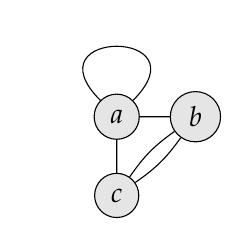
\begin{tikzpicture}
            [main/.style ={draw,circle}]
            \node[main][fill=gray!20!white] (a){$a$};
            \node[main][fill=gray!20!white] (b)[right of = a]{$b$};
            \node[main][fill=gray!20!white](c)[below of= a]{$c$};
            \draw (a) to (b) (c) to (a) (c) to [bend right =10](b) (c) to [bend left =10](b); 
            \draw (a) to [loop,red] (a);
        \end{tikzpicture} 
        \caption{graph $G(V,E)$ is an example of a graphs, the red edge is a loop, and all pair of vertices in this graph is adjecent.}
        \label{fig:graph}
    \end{subfigure}\hfill
   \begin{subfigure}{0.48\textwidth}
    \centering
        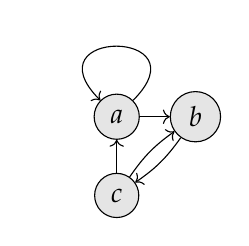
\begin{tikzpicture}
            [main/.style ={draw,circle}]
            \node[main][fill=gray!20!white] (a){$a$};
            \node[main][fill=gray!20!white] (b)[right of = a]{$b$};
            \node[main][fill=gray!20!white](c)[below of= a]{$c$};
            \draw[->] (a) to (b);
            \draw[->](c) to (a);
            \draw[->](c) to [bend left =10](b);
            \draw[->](b) to [bend left =10](c); 
            \draw[->] (a) to [loop,red] (a);
        \end{tikzpicture} 
        \caption{This is an oriantation of the edges in the graph which makes this a digraph}
        \label{fig:digraph}
   \end{subfigure}
\end{figure}


Before delving more specific into graphs and digraphs we must establish some important prerequisite and properties. 
A graph is called \textbf{simple} if there is no loops and no multiple edges. 
With multiple edges it means multiple edges between the same pair of vertices like in \autoref{fig:graph} between $b$ and $c$.
\begin{figure}[!h]
	\centering
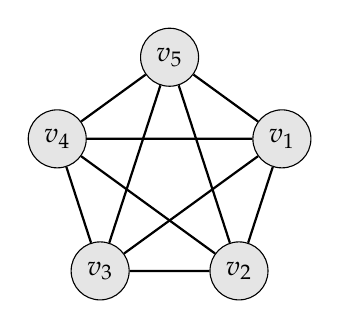
\begin{tikzpicture}[
	xs/.style = {xshift=#1 mm},
	ys/.style = {yshift=#1 mm}]
	
	\def \n {5}
	\def \radius {1.5cm}
	\def \margin {8} % margin in angles, depends on the radius
	
	\foreach \s in {1,...,\n}
	{
		\node[draw, circle][fill=gray!20!white] (\s) at ({360/\n * -(\s+3.75)}:\radius) {$v_\s$};
	}
    \draw[ thick] (1) -- (2) (1) -- (3) (1) -- (4) (1) -- (5);
    \draw[ thick] (2) -- (3) (2) -- (4) (2) -- (5);
    \draw[ thick] (3) -- (4) (3) -- (5);
    \draw[ thick] (4) -- (5);
    \end{tikzpicture}
\caption{Complete graph with 5 vertices.}
\label{fig:complete}
\end{figure}

A graph is \textbf{connected} if there exists a path between all pair of vertices in the graph and \textbf{disconnected} otherwise.
A graph is called \textbf{complete} if there for all pair of vertices in the graph is an edge between them see \autoref{fig:complete}.\\
Somtimes when looking at specifiks set of vertices we are actually interested in something called \textbf{independents set} which is a set of vertices of $G$ where there is no edge between the vertices in the set. A maximal independet set of $G$ is a independent set where you can not add any new vertex in the set that is not adjencent to any vertex in the set(adding a vertex makes the set no longer independent).  
A maximum independent set is the maximal independent set with greatest cardinality. 
Let $I\subset V$ be a maximum independet set then $|I|$ is called the \textbf{independence number}. \\ 

If we instead of edges have \textbf{arcs} between the vertices we call it a \textbf{digraph}.
An arc is describe just like an egde with two adjecent vertices $(a,b)$ the first vertex mentioned in an arc is the vertex \textbf{from} where the arc starts also called the \textbf{tail}, the second vertex is where the arc is pointing \textbf{to} also called \textbf{head}. The set of arcs is normaly denoted $A$ like the set of edges is denoted $E$ 
(so the arc $(a,b)$ goes from $a$ to $b$, if you wanted it the other way around the arc is $(b,a)$).
These graph contaning only arcs and no edges is called a digraph $D(V,A)$ which is what we in this project are focusing on see \autoref{fig:digraph}(as $G$ denote a \textbf{G}raph, $D$ denote a \textbf{D}igraph).\\
For two vertices $x$ and $y$ in $D(V,A)$ then if we have an arc from $x$ to $y$ we say that $x$ \textbf{dominates} $y$ this is denoted like this $x \rightarrow y$. If we talk about subgraphs $A$ and $B$, then $A$ \textbf{dominates} $B$ if for all $a\in A$ and $b\in B$, $a \rightarrow b$. If there is no arcs from $B$ to $A$ we denote it $A\mapsto B$ and if both $A\rightarrow B$ and $A \mapsto B$ we say that $A$ \textbf{completely dominates} $B$ and this is denoted $A\Rightarrow B$.\\ 

Sometimes when working with a digraph or solving a problem we have a subset of vertices $X\subseteq V(D)$ that want to work with as one vertex. 
Then we \textbf{contract} the vertecies $X$ into one vertex $x$ where $N^+(X)\backslash X=N^+(x)$ and $N^-(X)\backslash X=N^-(x)$ (so we only keep the ingoing and outgoing arcs of $X$ and delete all vertices of $X$ and the arcs inside). When we contract $X$ of $D$ we will try uding the notation $D/X$. There is also another kind of contraction where you also delete possible multiple arcs, if this is the case it will be explained in the section.\\

In a digraph we have something called the \textbf{underlying graph} denoted $UG(D)$. 
An underlying graph of a digraph is where all arcs are replaced by edges (edge is used every time we talk about undirected edges between vertices, when using directions it is called an arc).
Let $X \subseteq V$ Then we can make the subdigraph $D\left< X\right>$ which is the subgraph $D$ induced by the set $X$ meaning that all the vertices is from $X$ and the arcs is from $A\in G$ but where both head and tail is incedent to the vertices in $X$. 
We will denote the graph $D\left< V\backslash X\right>$ for some $X\subseteq V$ as $D-X$.
A digraph is \textbf{connected} if the underlying graph is connected, (also called weakly connected), a digraph can be \textbf{strongly connected} and \textbf{semi connected} too.
A digraph is called \textbf{semi connected} if there for each pair $u$ and $v$ exists a path from either $u$ to $v$ or $v$ to $u$.  
It is said to be \textbf{strongly connected} if for each pair of vertices $u$ and $v$ there exists a path from both $u$ to $v$ and $v$ to $u$. A strongly connected digraph is also called a \textbf{strong} digraph. 
A strong digraph have a subset $S$ called a \textbf{seperator} if $D-S$ is not strong, we also say that $S$ \textbf{seperates} $D$. 
A seperator $S$ is called \textbf{minimal seperator} of $D$ if there exists no proper subset $X\subset S$ that seperates $D$.
Now we can introduce a \textbf{$k$-strong} digraph $D$ which is a strong digraph where $|V|> k$ and a minimal seperator $S$ where $|S|= k$.
In the same way we can define $k$\textbf{-arc-strong} digraph is where you need to delete at least $k$ arcs for the digraph to no longer be strong. 

In a digraph $D(V,A)$ we mostly use the \textbf{dregree} as two different degrees namely \textbf{out degree}, $d^+(v)$, and \textbf{in degree}, $d^-(v)$, that is the arcs from $v$ and to $v$ respectively. 
In a digraph $D$ we can talk about the over all \textbf{minimum out degree}, $\delta ^+(D)=\min\lbrace d^+(v)|v\in V\rbrace$ and \textbf{minimum in degree}, $\delta ^-(D)=\min\lbrace d^-(v)|v\in V\rbrace$
somtime we are going to need the minimum of these to $\delta(D)=\min \lbrace\delta ^+(D),\delta ^-(D) \rbrace$ called the \textbf{minimum degree}.
For every vertex $v$ the vertices that is \textbf{adjacent} with $v$ is called \textbf{nieghbours} of $v$.
We denote $N^+(v)$ and $N^-(v)$ as the set of vertices that is dominated by (\textbf{out-nieghbours} of) $v$ and dominates (\textbf{in-nieghbours} of) $v$, respectivly. 
This means that $d^+(v)=|N^+(v)|$ and $d^-(v)=|N^-(v)|$.\\


For simplicity when mentioning paths and cycles in digraphs it will be \textbf{directed} paths and cycles if not anything else is mensioned. 
By \textbf{directed} means that we go from tail to head on every arc on the path or cycle.
When mentioning paths in a digraph it sometimes makes more sence specifing the head an tail of the path, so a path from $s$ to $t$ is denoted as an \textbf{($s,\ t$)-path}.
In some digraphs there is more than one path between the same two vertices these paths can use the same arcs or same vertices or be totally distinct from eachother, the maximum number of disjoint path between two vertices in a digraph is denoted $\lambda_D(s,t)$
 




\section{Computational complexity}
\label{sec:complexity}
In this section we will go over how time is measured for an algorithm and what it means for a problem to be polynomially solveable or polynomially verifyable. Also what it means for a problem to be NP-hard and NP-complete and how we found out if a problem is either of them. 

\subsection{Measure time of algorithm (Polynomial, exponential)}
The runing time of an algorithm is based on how many steps it is going thourgh which is somtimes based on the input that the algorithm takes we are going to denote an algorithms running time as a function $f(n)$ over the input $n$. 
This is how different functions can descirbe the running time of an algorithm, if an algorithm has the same number of steps no matter what the input is it has a constat running time where the constant is the number of steps the algorithm uses. 

An algorithm can also take the form of an polynomial function or even exponentiel, if this is the case we uses some notation as big-$O$ notation or $\theta$. 
Big-oh is the most used one and is the notation we are going to use in this thises, if the algorithm takes $f(n)=4n^3 +2n^2-n+2$ time we denote it in big-oh notation as $O(n^3)$ as it is the biggest term of $f(n)$.  

Since the shorter the runningtime is the better the algortihm is.
Since the exponentiel runningtime algortihms take forever on large inputs, we would want to improve them, but sometimes you are left with problems where that is not a possibility.

So we are going to classify the problems in gruops of how long time it take to decide or verify the problems solution. a problem that is decided i polynomiel time is in the class called $P$.
Which means for every given time of input in a problem from \textbf{P} we can find the solution for the problem in polynomiel time.

\subsection{NP problems and classifications}
As shortly described above there is something called a \textbf{polynomial verifier} for a problem. 
That means given a problem and then given a solution we can in polynomial time verify if it is a solution to the given problem. This is the class we call NP.
\begin{definition}
    \textbf{NP} is the class of languages that have polynomial time verifiers.
\end{definition}

Obiously if you can find a solution in polynomial time you can also verify whether a solution is correct in polynomial time. 
So $P\subseteq NP$. 
There is also a class called $NP-Hard$ but before we can explain that we need to explain what it means for a problem to be polynomial reduceable to another problem. 
For a specific problem $A$ and another problem $B$ then if there exists an algorithm that can take a solution from $A$ and make it a solution for $B$ in polynomial time. 
When such a algorithm exists it is called a polynomial verifier and we say that $A$ is \textbf{polynomial reducable} to $B$ or just that $A$ is \textbf{reduced} to $B$. 
\textbf{NP-Hard} are the class of problems that every NP problem can be polynomiel reduced to. 
A problems in the class of NP-Hard problems does not nessesarily mean that it is NP it-self.
If a problem is both \textbf{NP} and \textbf{NP-Hard} we call it \textbf{NP-Complete}. 
The problems we are \textcolor{red}{mostly} focusing on is in the class of \textbf{NP-Complete} problems.
   

\section{Classes of Digraphs}
\label{sec:class}
We can classefy specific collection of graphs the reason for this is that digraphs of smaller collections of digraphs (like tournaments is a smaller collection of semicomplete digraphs) might be because of problems that is hard to solve on general digraph but is \\
easy/polynomial solvable on specific types of digraphs.

A group of these problems is called NP-complete problems which sometimes sound easy solvable for graphs but only for some specific graphs we know how to solve it in polynomial time. 
Like finding paths in digraphs or cycles or more specific things, but in general des more we know about a digraph we can use to solve hard problems which in general would be time consuming like the problems that are NP-hard.
By some quick fast algorithm you can checks wheter a digraph belongs to a certion \textbf{class} of digraphs. 
A class of digraph is a collection of digraph with certain properties incommen like \textbf{tournaments}.\\
\subsection{introduction to some digraph classes}
\textbf{Tournaments} is a digraph where the underlying graph is complete. 
So a complete graph of order 5 any orientation of the edges concludes in a tournament.
Strong digraphs is also in it self a classification of digraphs. Classes of digraphs can be overlapping each other or be fully containt in each other like tournaments is fully containt in the class called semicomplete digraph.
A \textbf{semicomplete} digraph is where the underlying graph is complete multigraph, there can be some multiple edges in between the same pair of vertices in the underlying graph. Since the class called semicomplete digraphs contains all digraphs where the underlying graph is a complete multigraph it clearly also contains the graph with only one arc between every pair of vertecies (Tournaments).
A \textbf{complete} digraph is where every pair of vertices $a,b\in V$ the arc $(a,b)$ and $(b,a)$ is present in the graph. \\
If you can split the graph into two sets of vertices $A$ and $B$ such that $A\cup B=V$ and there is no arcs inside these sets, then we classify this as an \textbf{bipartite} digraph This means all arcs in the graph is in the form $(a,b)$ or $(b,a)$ for all $a\in A$ and $b\in B$. 
The sets $A$ and $B$ are called the partites of $D(V,A)$. 
The underlying graph of a bipartite digraph is also called bipartite since there is no edges inside $A$ or $B$.
If there exists more then two of these partite sets we call the digraphs \textbf{multipartite}, since there is multiple partite sets in the graph, bipartite sets $\subset$ multipartite. \\
A much used type of digraph is an \textbf{acyclic} digraph. 
It is a digraph where for an specific ordering of the vertices $V={v_1, v_2,\dots , v_n}$ the arcs in the digraph is $(v_i, v_j)$ where $i<j$ for all $(v_i, v_j)\in A$. This ordering is called an \textbf{acyclic ordering} and can also be used to order strong components in an non-strong digraph such that the ordering of the componentent $C_1,C_2,\dots C_k$ is an acyclic digraph when contracting the components into $k$ vertices. 
When classifying digraphs there is several ways of doing this, like \textbf{transitive} digraphs which are digraphs where for all vertices $a,d,c\in V$ where the arc $(a,b)$ and $b,c$ is present in the digraph ($\in A$), the arc $(a,c)$ has to be a part of $A$ too. 
using the same kind of classification there is digraphs which are \textbf{Quasi-transitive} which is forall vertices $a,d,c\in V$ where the arc $(a,b)$ and $b,c$ is present in the digraph ($\in A$), $a$ and $c$ has to be adecent by at \textit{least} one (more arcs in between are also allowed) arc in either direction ($(a,c)$ or $(c,a)$). These graphs are going to be mentioned a lot in this thises since the graph is also what we call \textbf{decomposable}.\\
\textbf{Decomposable} digraphs is also a clasification of graphs which are decomposable, for a graph $D$ to be decomposable we have $H_1,H_2, \dots , H_k$ \textbf{houses} and $S$ where $V(S)={s_1,s_2,\dots,s_k}$ which are all digraphs by them self but if each $s_i$ is replaced by the digraph $H_i$ $i=1,2,\dots,k$ we have the graph $D$, where $H_i\rightarrow H_j \in D$ if $s_i\rightarrow s_j\in S$  denote this decomposition like $D=S[H_1,H_2,\dots H_k]$.
This is the class of digraphs we are focusing on in this thises. 
If all the houses are independent sets we call $D=S[H_1,H_2,\dots ,H_k]$ the extension of $S$. 
If $S$ is a semicomplete digraph we call the extensin of these \textbf{extended semicomplete} digraph.
Like we already mentioned Quasi-transitive digraphs are decomposable but we have several classes that are decomposable, and another class of digraphs that is giong to be used a lot in this is \textbf{locally semicomplete} digraphs.\\
First we are going to introduce \textbf{in-locally semicomplete} digraphs and \textbf{out-locally semicomplete} digraphs which is for every in-nieghboor of a vertex $x\in V$ they have to be adjecent ($x\cup N^-(x)$ induces a semicomplete digraph) is the in-locally semicomplete digraph if it is true for all $x\in V$. 
Respectively it is called an out-locally semicomplete digraph if $\forall x\in V$ the out-nieghboors, $N^+(x)$, has to be adjecent. 
If a digraph is both in-locally semicomplete and out-locally semicomplete, it is called a \textbf{locally semicomplete} digraph. Why both Quasi transitive digraphs and some locally semicomplete digraphs are decomposeble will be described in section \autoref{sec:Decomposable}.\\
The last class of digraph that are important for this thises is the round digrphs. 
A digraph is called a \textbf{round} digraph if there exists an ordering of the vertices $v_1,v_2,\dots,v_n$ such that for all $v_i$, $N^+(v_i)={v_{i+1},v_{i+2},\dots ,v_{i+d^+(v_i)}}$ and $N^-(v_i)={v_{i-d^-(v_i)},v_{i-(d^-(v_i)-1)},\dots ,v_{i-1}}$.






\chapter{Decomposable Digraphs}
\label{chap:decomposable}
Decomposable digraphs is what we in this thesis is focusing on. 
We have introduced short what a decomposable digraph is but there is subclasses to focus on and a lot of other crucial definitions and theroems to cover about these digraphs before delving into the NP-hard problems. 
First we cover some general things about decomposable digraphs the next section is about quasi-transitive digraphs, and why they are a subclass of decomposable digraphs and $\phi_1$-decomposable digraphs. At the end of the section we prove that these decompositions can be found in polynomial time. 
Which is going to be crucial for solving some NP-hard problems for this class of digraphs. Then we are going to look at a very general class of digraphs locally semicomplete digraphs, where this class can be split up to 3 different subclasses where 2 of those are decomposable. 
This is covered in \autoref{sec:locally} and is going to be used in later chapthers. 
\section{General about Decomposable digraphs}
\label{sec:gdecomposable}
Recall that a decomposable digraph $D$ can be decomposed into a main graph $S$ where $|S|=k$ and $k$ houses $H_1,H_2,\dots , H_k$, where each vertex in $S=\lbrace v_1,v_2\dots ,v_k\rbrace$ is replaced by the house $H_i$ replace $v_i$ and the arcs between the houses is as follows $H_i \rightarrow H_j$ in $D$ if $v_i\rightarrow v_j$ in $S$ remember that for a set $X$ to dominate an other set $Y$ (meaning every vertex in the dominating set dominates every vertex in the dominated set) we denoted it $X \rightarrow Y$. If no arc between $v_a$ and $v_b$ in $S$ then there is no arc between the sets $H_a$ and $H_b$ in $D$. 
The thing about decomposable digraphs is that if there is an arc between $H_i$ and $H_j$ either one of the houses totally dominates the other (ex. $H_i \Rightarrow H_j$) or they dominate each other (ex. $H_i \rightarrow H_j$ and $H_j\rightarrow H_i$).

Decomposable digraphs can be classed by a set of digraphs $\phi$, when \\
$D=S[H_1,H_2,\dots ,H_k]$ it is \textbf{$\phi$-decomposable} if $D\in \phi$ or if $S\in \phi$. The chioces of $H_i$ for $i=1,2\dots , k$ does not determine anything about the digraph being $\phi$-decomposable but the class of \textbf{totally $\phi$-decomposable} digraphs is where $D$ is $\phi$-decomposable and each $H_i$ is totally $\phi$-decomposable. 
We are going to make two shuch sets of digraphs $\phi_1$ which is the union of semicomplete digraph and acyclic digraph both classes deskribed in \autoref{sec:class} and $\phi_2$ which is the union of semicomplete and round digraphs also deskribed in \autoref{sec:class}.  
\begin{align}
    \phi_1=\text{Semicomplete digraphs}\cup \text{Acyclic digraphs}
    \label{eq:phi1}\\
    \phi_2=\text{Semicomplete digraphs}\cup \text{Round Digraphs}
    \label{eq:phi2}
\end{align}

\section{Quasi-transitive Digraph}
\label{sec:quasi}
First we need to recall what a quasi transitive digraph is. 
For every triplet $x,y,z$ in a quasi-transitive digraph if $x\rightarrow y$ ($x$ dominates $y$) and $y\rightarrow z$ ($y$ domitaes $z$), then there has to be at least one arc in either dirction between $x$ and $z$. 
When working with quasi-transitive digraphs there are many things you can depend on, things that the structure has already diceded for us.
\begin{lemma}~\cite{banggutin}
    Suppose that $A$ and $B$ are distinct strong components of a quasi-transitive digraph $D$ with at least one arc from $A$ to $B$. Then $A\rightarrow B$.
    \label{lemma:dominatingset}
\end{lemma}
Recall that this means that every vertex in $A$ has an arc to every vertex in $B$.
Like non-strong quasi-transitive digraph we can also say something about strong quasitransitive digraphs.
\begin{lemma}~\cite{banggutin,bangJGT2}
    Let $D$ be a strong quasi-transitive digraph on at least two vertices. Then the following hold:
    \begin{itemize}
        \item[(a)] $\overline{UG(D)}$ is disconnected;
        \item[(b)] If $S$ and $S'$ are two subdigraphs of $D$ such that $\overline{UG(S)}$ and $\overline{UG(S')}$ are distinct connected components of $\overline{UG(D)}$, then either $S\rightarrow S'$ or $S'\rightarrow S$ or both $S\rightarrow S'$ and $S'\rightarrow S$ in which case $|V(S)|=|V(S')|=1$. 
    \end{itemize} 
    \label{lemma:underlyinggraph}
\end{lemma}
These to lemmas is also a part of proving the one theorem which states that quasi-transitive digraphs can be decomposed no matter if there are strong or nonstrong digraphs. 

\begin{thm}\cite{bangJGT85}
    Let $D$ be a quasi-transitive digraph.
    \begin{enumerate}
        \item If $D$ is not strong, then there exists a transitive acyclic digraph $T$ on $t$ vertices and strong quasitransitive digraphs $H_1,\dots,H_t$ such that $D=T[H_1,\dots,H_t]$.
        \item If $D$ is strong, then there exists a strong semicomplete digraph $S$ on $s$ vertices and quasitransitive digraphs $Q_1,\dots ,Q_s$ such that each $Q_i$ is either a single vertex or is nonstrong and $D=S[Q_1,\dots,Q_s]$.
    \end{enumerate}
    \label{thm:quasidecom}
\end{thm}
This theroem is also what we are going to use more then ones, to prove several of the problem solving theorems through out this thises.
\begin{proof}
    Since we can decompose both strong quasi-transitive digraphs and non-strong quasi-transitive digraph we are going to prove if $D$ is not strong first and there after if $D$ is strong.
    So suppose $D$ is not strong, then we know we can enumerate the strong components in an acyclic order let these be $H_1,\dots , H_t$. \\
    Recall that an acyclic ordering of the strong components does not mean that there is no arcs going back in the ordering, but we will prove that now. \\
    Now from \autoref{lemma:dominatingset} we know that if there is an arc between two of the strong components, one of them dominates the other.
    Let with out loss of generality these set be $H_i$ and $H_j$ and let $H_i\rightarrow H_j$. 
    Then Since $D$ is not-strong $H_j\nrightarrow H_i$ now let say that $H_j \rightarrow H_k$, then since $D$ is quasi-transitive then either $H_k\rightarrow H_i$ or $H_i \rightarrow H_k$. 
    But since $H_i\cup H_j \cup H_k$ is not strong $H_k\nrightarrow H_i$ meaning contracting each $H_i$ for $i=1\dots,t$ we will have a transitive digraph $T$ and we have also shown that there are no backwards going arcs in the ordering meaning that $T$ is not only transitive but acyclic. 
    This end the proof of the non-strong quasi-transitive digraph leving only the strong ones left.\\

    Now suppose that $D$ is a strong quasi-transitive digraph, we now look at the underlying graph $UG(D)$ after this we find the complement of it, $\overline{UG(D)}$ since $D$ is strong we know from \autoref{lemma:underlyinggraph} that $\overline{UG(D)}$ is disconnected, so we find $Q_1,\dots , Q_s$ where $\overline{UG(Q_i)}$ is connected in $\overline{UG(D)}$ $\forall i \in [s]$.\\ 
    Since these subdigraphs $\overline{UG(Q_i)}$ of $\overline{UG(D)}$ is connected we know that $Q_i$ is non-strong or a single vertex in $D$. 
    From the same lemma each $Q_i$ (reprecent $S$ in \autoref{lemma:underlyinggraph}) which means when contracting $Q_i$ $\forall i\in [s]$ into a single vertex $q_i$. 
    Denote $D$ with contracted $Q_i$'s as $S$. 
    We have that every pair of vertex in $S$ have one arc between in either direction or one in both direction making $S$ semicomplte. \\
    This concludes the proof.
\end{proof}
From this theorem we can see that quasi-transitive digraphs is totally $\phi_1$-decomposable. 
Since the transitive digraph for the nonstrong quasi-transitive digraphs is acyclic $T\in \phi_1$ and each $H_i$ is itself strong quasi-triansitive digraphs and you can therefore use \autoref{thm:quasidecom} agian.  
For the strong quasi-transitive digraphs $D$, $S$ is semicomplete so $S\in \phi_1$ and each $Q_i \in \phi_1$ because it is either one vertex which is a digraph that is both acyclic and semicomplete or it is non-strong and must be quasi-transitive and therefore \autoref{thm:quasidecom} can be used agian. So every nonstrong and strong quasi-transitive digraphs is totally $\phi_1$-decomposable.

\begin{thm}
    \textcolor{red}{quasi decomposition can be found in poly time}
\end{thm}

\section{Locally semicomplete Digraph}
\label{sec:locally}
blablabla
\begin{thm}
    \textcolor{red}{round decompose locally semicomplete digraph}
\end{thm}
Every locally semicomplete digraph can be classified into some other groups of digraphs namely semicomplete digraphs and round decomposable digraphs and the last one which is neither of the two is call evil. Round decomposable digraph $D=R[D_1,\dots,D_r]$ is where $R$ is a round digraph of the strong componentents $D_i$ and $|R|=r$.
\begin{thm}~\cite{bangJGT85}
    Let $D$ be a locally semicomplete digraph. Then exactly one of the following possibilities holds. Furthermore, there is a polynomial algorithm that decides which of the properties hold and gives a certificate for this.
    \begin{itemize}
        \item[(a)] $D$ is round decomposable with a unique round decomposition $R[D_1,\dots ,D_r]$, where $R$ is a round local tournament on $r\geq 2$vertices and $D_i$ is strong semicomplete digraph for $i=1,2,\dots,r$.
        \item[(b)] $D$ is evil 
        \item[(c)] $D$ is a semicomplete digraph thet is not round decomposable. 
    \end{itemize}
\end{thm}
If the locally semicomplete digraph is nonstrong it turns out that it is decomposable this is called a semicomplete decomposition.
\begin{thm}~\cite{bangJGT85,banggutin,bangJCT102}
    Let $D$ be a nonstrong locally semicomplete digraph and let $D_1,D_2,\dots,D_p$ be the acyclic order of the strong components of $D$. Then $D$ can be decomposed into $r\geq 2$ disjoint subdigraphs $D_1',D_2',\dots, D_r'$ as follows:
    \begin{align*}
        D_1'=D_p, \lambda_1=p,\\
        \lambda_{i+1}=min\lbrace j|N^+(D_j)\cap V(D'_i)\neq \emptyset\rbrace,
    \end{align*}
    and
    \begin{equation*}
        D'_{i+1}=D\left<V(D_{lambda_{i+1}})\cup V(D_{lambda_{i+1}+1})\cup \cdots \cup V(D_{lambda_{i}-1})\right>
    \end{equation*}
    The subdigraphs $D'_1,D'_2,\dots,D'_r$ satisfy the properties below:
    \begin{itemize}
        \item[(a)] $D'_i$ consists of some strong components that are consecutive in the acyclic ordering of the strong components of $D$ and is semicomplete for $1=1,2,\dots,r$;
        \item[(b)] $D'_{i+1}$ dominates the initial component of $D'_i$ and there exists no arc from $D'_i$ to $D'_{i+1}$ for $i=1,2,\dots,r-1$;
        \item[(c)] if $r\geq 3$ then there exists no arc between $D'_i$ and $D'_j$ for $i,j$ satisfying $|j-i|\geq 2$  
    \end{itemize}
    \label{thm:semicompletedecom}
\end{thm}
For simplification of \autoref{thm:semicompletedecom} the properties is drawn out in \autoref{fig:properties}
\begin{figure}
    \begin{tikzpicture}
        \node[$a$](a)
    \end{tikzpicture}
    \caption{(a)(b) and (c)}
    \label{fig:properties}
\end{figure}
Now we focus more on the structure of the evil locally semicomplete digraph which we have not covered jet, there is a fine understanding of the structure of round decomposable and the semicomplete digraphs, even the semicomplete decomposition which is a part of the evil structure too.
First we have to recall what a minimal seperator from \autoref{sec:digraph}, then use this to construct what we call a \textbf{good} seperator.
\begin{lemma}~\cite{bangJGT85}
    Let $S$ ba a minimal seperator of the locally semicomplete digraph $D$. Then either $D\left< S\right>$ is semicomplete or $D\left< V-S\right>$ is semicomplete.
    \label{lem:whichsemicomplete}
\end{lemma}
Then a \textbf{good} seperator of a locally semicomplete digraph is minimal and $D\left<V-S\right>$ is not semicomplete.
When finding a good seperator in a evil locally semicomplete digraph, then the part that is left $D-S$ a semicomplete decomposition can be found it turns out that there is a lot to say about this decomposition.
\begin{thm}~\cite{bangJGT85,bangJCT102}
    Let $D$ be an evil locally semicomplete digraph then $D$ is strong and satisfies the following properties.
    \begin{itemize}
        \item[(a)]There is a good seperator S such that the semicomplete decomposition of $D-S$ has exactly three components $D'_1,D'_2,D'_3$ (and $D\left<S\right>$ is semicomplete by \autoref{lem:whichsemicomplete});
        \item[(b)] Furthermore, for each such $S$, there are integers $\alpha, \beta,\mu,\nu$ with $\lambda_2\leg \alpha \leq \beta \leq p-1$ and $p+1\leq \mu \leq \nu \leq p+q$ such that 
        \begin{align}
            &N^-(D_\alpha)\cap V(D_\mu)\neq \emptyset \text{and} N^+(D_\alpha)\cap V(D_\nu)\neq \emptyset,\\
            \text{or} &N^-(D_\mu)\cap V(D_\alpha)\neq \emptyset \text{and} N^+(D_\mu)\cap V(D_\beta)\neq \emptyset,
        \end{align} 
        where $D_1,D_2,\dots, D_p$ and $D_{p+1},\dots,D_{p+q}$ are the strong decomposition of $D-S$ and $D\left< S\right>$, respectively, and $D_{\lambda_2}$is the initial component of $D'_2$ 
    \end{itemize}
    \label{thm:evildecom}
\end{thm}
Even though this is a structure we can work with, we can actually go deeper into the structure of this evil locally semicomplete digraph. Namly trying to group the components inside the semicomplete decomposition $D'_1,D'_2,D'_3$ and the good seperator $S$. This structer is menation in \cite{bangJGT85} but also in \cite{tildeDMCS}. First we can establish this lemma which is a big part of the structure of evil locally semicomplete digraphs.
\begin{lemma}~\cite{tildeDMCS}
    Let $D$ be an evil locally semicomplete digraph and let $S$ be a good seperator od $D$. Then the following holds:
    \begin{itemize}
        \item[(i)] $D_p\Rightarrow S\Rightarrow D_1$.
        \item[(ii)] If $sv$ is an arc from $S$ to $D'_2$ with $s\in V(D_i)$ and $v\in V(D_j)$, then 
        \begin{equation*}
            D_i\cup D_{i+1}\cup \dots D_{p+q}\Rightarrow D_1\cup\dots \cup D_{\lambda_2-1}\Rightarrow D_\lambda_2\cup \dots \cup D_j
        \end{equation*}.
        \item[(iii)] $D_{p+q}\Rightarrow D'_3$ and $D_f\Rightarrow D_{f+1}$ for $f\in [p+q]$, where $p+q+1=1$.
        \item[(iv)] If there is any arc from $D_i$ to $D_j$ with $i\in [\lambda_2-1]$ and $j\in [\lambda_2,p-1]$, then $D_a\Rightarrow D_b$ for all $a\in [i,\lambda_2-1]$ and $b\in[\lambda_2,j]$.
        \item[(v)] If there is any arc from $D_k to D_l$ with $k\in [p+1,p+q]$ and $l\in [\lambda_2-1]$, then $D_a\Rightarrow D_b$ for all $a\in [k,p+q]$ and $b\in [l]$.   
    \end{itemize}
\end{lemma}


\chapter{Path cover and hamilton cycles}
\label{chap:hamilton}
In this chapter the focus is the hamilton cycle problem, where we know that if we can solve the path covering problem then we can solve the hamilton cycle problem for quasi-transitive digraphs.\\
In the first section we are going to cover, what a hamilton path is, and a hamilton cycle Since these to problems are well know as \textbf{NP-Complete} which will shortly be introduced too.\\
The next section is about path-mergeable digraphs and that locally semicomplete digraphs are a subclass of these and how this helps in the path covering problem and hamilton cycle problem. 
%Then state some theorems that says knowing special things about the graph we know when it contain a hamilton cycle. \\
The following section is covering quasi-transitive digraphs and whether or not there exists a hamilton cycle in those. Here the decomposition of the quasi-transitive digraphs is going to be a crucial part of proving this. \\


\section{The Hamilton Path and Cycle Problem}
\label{sec:hNP}
Finding a hamilton cycle in a digraph is a well know problem, but here is a shortly explanaition of what that is.
When we define what a hamiltonian digraph is we first have to explain what a hamilton cycle is. A hamilton cycle is a directed cycle $C_H$ in a digraph that contains(pass by) every vertex in the digraph $\forall v\in V(D), v$ is in $C_H$.\\
\begin{definition}
    A Hamiltonian digraph is a graph containing a hamilton cycle 
\end{definition} 
We can also define digraphs called traceable
\begin{definition}
    A traceable digraph is a digraph containing a hamilton path
\end{definition}
A hamilton path is a path containing all vertices of the digraph.\\
The problems that is considered \textcolor{red}{NP-Hard} is finding out whether an arbitrary digraph is trecable or hamiltonian. 
We are going to show that hamilton cycle problem is \textcolor{red}{NP-Hard} by reducing it to a problem we know is. 
Then we are going to show that if we know that a digraph is traceable it takes polynomial time to figure out wheter it is hamiltonian too, making the traceable problem \textcolor{red}{NP-Hard} too. 
Because if the you in polynomial time could figure out wheter a arbitrary digraph is traceable you know that if it is not, it is defenatly not hamiltonian. 
And if it is you can in polynomial time figure out if it is hamiltonian, making the hamton cycle problem a polynomial time solution problem (not \textcolor{red}{NP-Hard}). 
\section{Hamiltonian Locally semicomplete Digraphs}
\label{sec:hlocally}
Recall that a locally semicomplete digraph is both in-locally semicomplete and out-locally semicomplete. 
Before this gets relevant we are going to introduce a class of digraphs called path-mergeable they are not introduced under section \autoref{sec:class} since we are only going to use it in this section.
A short explanaition of a path mergeable digraph is that it is the class of digraphs where given two paths with the start- and endpoint incommen you can merge the two paths into one using all vertices in the two paths. 
A more formal definition of path mergeable digraphs is if there exists a pair of distinct vertices $x,y\in V(D)$ and any two disjoint $(x,y)$-paths there exists a new path from $x$ to $y$ where it is a union of the vertices used in the two vertex-disjoint paths (ending up with a "merge" path of the two given path).\\
These digraphs are easy to regonize with the following corolary we can do it in polynomial time too and the following theroem gives us a nice propertie of path-mergeable digraphs.
\begin{cor}~\cite{banggutin}
    Path-mergeable digraphs can be regonized in polynomial time
\end{cor}
\begin{thm}~\cite{banggutin}
    A digraph $D$ is path mergeable if and only if for every pair of distict vertices $x,y\in V(D)$ and every pair $P=xx_1\dots x_ry,\ P'=xy_1\dots y_sy$, $r,s\geq 1$ of internally disjoint $(x,y)$-paths in $D$, either there exists an $i\in \lbrace 1,\dots ,r\rbrace$, such that $x_i\rightarrow y_1$, or there exists a $j\in \lbrace 1,\dots, y_j\rightarrow x_1\rbrace$.
    \label{thm:pathmerge}
\end{thm}
to explain this \autoref{thm:pathmerge} it tells us that for every path mergeable digraph in every two disjoint $(x,y)$-path there has to be from one of the path a vertex that dominates the first vertex after $x$ in the other path. This has to hold for every distict pair of vertices $x$ and $y$. \\
It turns out that in these digraph we can easily determine whether it is a hamiltonian digraph too.
\begin{thm}
    A path-mergeable digraph $D$ of order $n\geq 2$ is hamiltonian if and only if $D$ is strong and $UG(D)$ is $2$-connected.
    \label{thm:pathham}
\end{thm}
\begin{cor}
    There is an $O(nm)$-algorithm to decide whether a given strong path-mergeable digraph has a hamiltonian cycle and find one if it exists.
    \label{cor:polypath}
\end{cor}
So it turns out that for path-mergeable digraphs this problem is polynomial solveable, and a subclass of these path-mergeable digraph is namely the locally semicomplete digraphs. If we can prove this we only know that we can solve the hamilton cycle in polynomial time and since the locally semicomplete digraphs is a subclass of in-locally semicomplete digraphs we have an even better time for these.
\begin{prop}
    Every locally in-semicomplete (out-semicomplete) digraph is path-mergeable.
\end{prop}
\begin{proof}
    proof this ... ... ... ... ... ... ... 
\end{proof}

Then it turns out that \autoref{thm:pathham} and \autoref{cor:polypath} can be imporved if we are only looking at the in-locally semicomplete digraph, since the locally semicomplete digraph is a subclass of these, and it is the ones we are interested in, in this thises. It turns out that every strong in-locally semicomplete digraph has a 2-connected underlyning graph, which means the only thing we need to check is whether it is a strong digraph.
\begin{thm}
    A locally in-semicomplete digraph $D$ of order $n\geq 2$ is hamiltonian if and only if $D$ is strong.
\end{thm}

It turns out that when looking at the strong locally in-semicomplete digraphs out of the path-mergeable digraph finding the hamiltonian cycle can be done i polynomial time by theorem discorvered by ... ...
\begin{thm}
    There is an $O(m+n\text{log}n)$-algorithm for finding a hamiltonian cycle in a strong locally in-semicomplete digraph.
\end{thm}


\section{Hamiltonian Quasi-transitive Digraphs}
\label{sec:hquasi}
First of all we have to recall \autoref{thm:quasidecom} since it is the key theorem to solve the hamiltonian problem in polynomial time. \\
Remember that a condition for a digraph to be hamiltonian is that it need to be strong, so for finding a hamilton cycle in a quasi-transitive digraph, we are not interested in the non-strong digraphs. 
Leving only the strong quasi-transitive digraphs with decomposition $S[Q_1,\dots Q_s]$ from \autoref{thm:quasidecom}. 
The given decomposition of strong quasi-transitive digraphs has a semicomplete digraph as the quotient. This is why we need some inside to these before the main solution in this subsection can be proven. another composition of semicomplete digraphs is the extension of these, called extended semicomplete digraph. An extension of a digraph is a composition of the given digraph $S$ where the hauses of the composition is either a single vertex or independence sets. \\
Before we explain when we can find a hamilton cycle in strong quasi-transitive digraphs we need to recall what a cycle factor is. 
From \autoref{sec:digraph} we shortly explain that a cycle factor is when we can find $C_1,\dots C_k$ cycles in $D$ contaning all vertices of $D$. 
\begin{thm}~\cite{gutinMNN2}
    An extended semicomplete digraph $D$ is hamiltonian if and only if $D$ is strong and contains a cycle factor. One can check whether $D$ is hamiltonian and construct a Hamilton cycle of $D$ (if one exsists) in time $O(n^{2.5})$.
    \label{thm:extended}
\end{thm}
\begin{thm}~\cite{bangJGT20}
    A strong quasi-transitive digraph $D$ with a canonical decomposition \\$D=S[Q_1\dots, Q_s]$ is hamiltonian if and only if it has a cycle factor $\mathcal{F}$ such that no cycle of $\mathcal{F}$ is a cycle of some $Q_i$.
    \label{thm:qhcycle}
\end{thm}
\begin{proof}
    Since a hamiltonian cycle need to cover all vertices in a digraph, we know that it must cross every $Q_i$. 
    Moreover the hamilton cycle is a cycle factor not fully containt in any $Q_i$. So we only need to show that if we have a cycle factor $\mathcal{F}$, where no cycle is in any $Q_i$, then $D$ is hamiltonian. $\forall i$ $V(Q_i)\cap \mathcal{F}=\mathcal{F}_i$, there can not be any circle in this and since every vertex is in $\mathcal{F}$ all vertices in $Q_i$ must be containt in $\mathcal{F}_i$ and there is no cycle containt in $\mathcal{F}_i$ whcich makes it a path factor of $Q_i$.\\
    \textcolor{red}{Figure here}\\
    For all paths in $\mathcal{F}_i$ we make a path contraction. 
    After contraction or before we delete the remaining arcs if this is done before its the arcs going from the end of a path to a begining of an other path. This action will make $Q_i$ an independent set $\forall i\in [s]$. Since $S$ is a semicomplete digraph our new digraph would then because of the independence of each $Q_i$ after the action be an extended semicomplete digraph $S'$. 
    Since we have only made path contractions along the cycles in the cycle factor of $D$ and not deleted any arcs that are a part of the cycle factor $S'$ contains a cycle factor. 
    Then by \autoref{thm:extended} we know that $S'$ contains a hamilton cycle. Adding the deleted arcs does not change this insert a path instead of a node just makes the cycle longer but it still contains every vertex given a hamilton cycle in $D$
\end{proof}

A hamilton path does not have the same condition for a digraphs to be strong meaning we are also interested in the non-strong quasi-transitive digraphs $T[H_1,\dots ,H_t]$. 
The next theorem is proven in much the same as \autoref{thm:qhcycle}. 
\begin{thm}~\cite{bangJGT20}
    A quasi-transitive digraph $D$ with at least two vertices and with canonical decomposition $D=R[G_1,G_2,\dots , G_r]$ is traceable if and only if it has a $1$-path-cycle factor $\mathcal{F}$ such that no cycle or path of $\mathcal{F}$is completely in some $D\left< V(G_i)\right>$.
\end{thm}

We know that the canonical decomposition of a quasi-transitive digraph can be found i polynomial time. 
We can also find the hamilton cycle in a quasi-transitive digraph in polynomial time, but also verify if it does not exists for the given graph. This result was proved by Gutin. ... 

\begin{thm}~\cite{banggutin94}
    There is an $O(n^4)$ algorithm which, given a quasi-transitive digraph $D$, either returns a hamiltonian cycle in $D$ or verifies that no such cycle exists.
\end{thm}






	\clearpage
	\part{Linkage and weak linkage}
	\clearpage
	\part{Spanning disjoint subdigraphs (Arc decomposition)}
	\clearpage
\bibliographystyle{unsrt}
\bibliography{bib}
\end{document}